\documentclass[11pt]{article}
\setlength{\oddsidemargin}{12pt}
\setlength{\textwidth}{6.5in}
\setlength{\textheight}{9in}
\pagestyle{empty}
\setlength{\parskip}{7pt plus 2pt minus 2pt}
\usepackage{amsmath}
\usepackage{graphicx}
\graphicspath{{.}}

\begin{document}

    \begin{center}
    {{\large CS 230 : Discrete Computational Structures}}
        \\

%\vspace*{1cm}

        {\bf Spring Semester, 2021}\\

        {\sc Homework Assignment \#8}\\
        {\bf Due Date:}  Wednesday, Apr 7
    \end{center}

    \noindent {\bf Suggested Reading:} Rosen Sections 5.3; Lehman et al. Chapters 5, 6.1 - 6.2, 7

    For the problems below, explain your answers and show your reasoning.

    \begin{enumerate}

        \item {\bf [8 Pts]} Prove that $f_0 - f_1 + f_2 - \cdots - f_{2n-1} + f_{2n} = f_{2n-1} - 1$ where $f_i$ are the Fibonacci numbers.
        \begin{enumerate}
            \item Base case: k = 1, $f_0 - f_1 + f_2 = f_1 - 1$ aka $0 - 1 + 1 = 1 - 1 = 0$
            \item Induction Hypothesis: $f_0 - f_1 + f_2 - \cdots - f_{2k-1} + f_{2k} = f_{2k-1} - 1$
            \item Prove: $f_0 - f_1 + f_2 - \cdots - f_{2k-1} + f_{2k} - f_{2(k + 1)-1} + f_{2(k + 1)} = f_{2(k + 1)-1} - 1$
            \item $(f_{2k-1} - 1) - f_{2(k + 1)-1} + f_{2(k + 1)} = f_{2(k + 1)-1} - 1$ \null\hfill IH
            \item $f_{2k-1} - f_{2k + 1} + f_{2k + 2} = f_{2k + 1}$
            \item $f_{2k-1} - f_{2k + 1} + (f_{2k + 1} +f_{2k}) = f_{2k + 1}$ \null\hfill $f_{2k + 2} = f_{2k + 1} +f_{2k}$
            \item $(f_{2k-1} + f_{2k}) = f_{2k + 1}$
            \item $f_{2k + 1} = f_{2k + 1}$ \null\hfill QED
        \end{enumerate}
        \item {\bf [12 Pts]} Let $S$ defined recursively by (1) $4 \in S$ and (2) if $s \in S$ and $t \in S$, then $st \in S$. Let $A = \{4^i \mid i \in {\cal Z}^+\}$. Prove that

        \begin{enumerate}

            \item {\bf [6 Pts]} $A \subseteq S$ by mathematical induction.
            \begin{enumerate}
                \item Base case: k = 1, $4^1 = 4 \in S$
                \item Induction Hypothesis: $s, t \in S$, $4^k = st \in S$
                \item Prove: $x, y \in S$, $4^{k+1} = xy \in S$
                \item $4*4^k = xy$
                \item $4*st = xy$ \null\hfill IH
                \item $4 \in S$ and $st \in S$, so $xy, 4^{k+1} \in S$ \null\hfill QED
            \end{enumerate}

            \item {\bf [6 Pts]} $S \subseteq A$ by structural induction.
            \begin{enumerate}
                \item Base case: $4 = 4^1$, so $4 \in S$ and $4 \in A$
                \item Induction Hypothesis: $x, y \in S$, assume $x, y \in A$. By (2), $xy \in S$
                \item Prove: $xy \in A$
                \item $x, y \in A$, so $x = 4^a$, $a \in Z^+$ and $y = 4^b$, $b \in Z^+$ \null\hfill IH
                \item $xy = 4^{a + b}$, $a + b \in Z^+$. Therefore, $xy \in A$ \null\hfill Def. of A; QED
            \end{enumerate}

        \end{enumerate}

        \item {\bf [5 Pts]} Define the set $S = \{2^k 3^m 5^p\mid k,m,p \in \cal Z\}$ inductively. You do not need to prove that your construction is correct. \\
        Basis: $k, m, p = 0$, $1 \in S$ \\
        Inductive Step: if $a \in S$ and $b \in$ \{2, 3, 5\}, then $ab \in S$

        \item {\bf [10 Pts]} Consider the following state machine with five states, labeled 0, 1, 2, 3 and 4. The start state is 0. The transitions are $0 \rightarrow 1$, $1 \rightarrow 2$, $2 \rightarrow 3$, $3 \rightarrow 4$, and $4 \rightarrow 0$.

        Prove that if we take $n$ steps in the state machine we will end up in state 0 if and only if $n$ is divisible by 5. Argue that to prove the statement above by induction, we first have to {\it strengthen the induction hypothesis}. State the strengthened hypothesis and prove it.
        \begin{enumerate}
            \item Predicate: P(n): After n steps, the state machine is in state 0 iff n is divisible by 5.
            \item Basis: $5\;|\;0$, so P(0) is true
            \item Inductive Step: Assume P(k)
            \item Prove: P(k + 1)
            \item Suppose $5\;|\;k$. By IH, statemachine is in 0 after k steps. However, $5 \not|\;k + 1$ because the state machine is in state 1 after k + 1 steps. State machine is in state 0 after k + 1 steps iff $5\;|\;k + 1$. Both are false, therefore P(k + 1)
            \item Should $5 \not|\;k$, By IH, state machine is in state 1, 2, 3, or 4. We cannot know if going 1 step after k steps will result in state 0. We need a stronger hypothesis to account for the other states.
            \item Stronger Induction Hypothesis: P(n): After n steps, the state machine is in state p, where p = n \% 5.
            \item Prove $\forall n, P(n)$
            \begin{enumerate}
                \item Basis: n = 0, state machine is in state 0 and $0 = 0 \% 5$
                \item Induction Steps:
                \begin{enumerate}
                    \item Case 1: k \% 5 = 0, By IH, in state 0 after k steps.
                    \item Case 2: k \% 5 = 1, By IH, in state 1 after k steps.
                    \item Case 3: k \% 5 = 2, By IH, in state 2 after k steps.
                    \item Case 4: k \% 5 = 3, By IH, in state 3 after k steps.
                    \item Case 5: k \% 5 = 4, By IH, in state 4 after k steps.
                \end{enumerate}
                \item Proof by Case:
                \begin{enumerate}
                    \item Case 1: k + 1 \% 5 = 1, By IH, in state 1 after k + 1 steps.
                    \item Case 2: k + 1 \% 5 = 2, By IH, in state 2 after k + 1 steps.
                    \item Case 3: k + 1 \% 5 = 3, By IH, in state 3 after k + 1 steps.
                    \item Case 4: k + 1 \% 5 = 4, By IH, in state 4 after k + 1 steps.
                    \item Case 5: k + 1 \% 5 = 0, By IH, in state 5 after k + 1 steps.
                \end{enumerate}
            \end{enumerate}
        \end{enumerate}
        \newpage
        \item {\bf [10 Pts]} A robot wanders around a 2-dimensional grid. He starts out at (0,0) and can take the following steps: (-1,+3), (+2,-2) and (+4,0).
        Define a state machine for this problem. Then, define a Preserved Invariant and prove that the robot will never get to (2,0).
        \begin{center}
            States: $\{ (a,b)\;|\; a, b \in Z\}$, Transitions: $\{ (a, b) \to (a - 1, b + 3), (a, b) \to (a + 2, b - 2), (a, b) \to (a + 4, b)\}$
        \end{center}
        \begin{enumerate}
            \item Preserved Invariant Theorem: For every reachable state $s = (a, b)$, $(a - b)\;\%\; 4 = 0$
            \item Basis: $(0, 0)$ is reachable in 0 steps.
            \item Induction Hypothesis: Assume $(r_1 - r_2)\;\%\; 4 = 0$ for any state $r = (r_1, r_2)$ that is reachable in k steps.
            \item Prove: $(s_1 - s_2)\;\%\; 4 = 0$ for any state $s = (s_1, s_2)$ that is reachable in k + 1 steps.
            \item $r_1 - r_2 = 4n$, $n \in Z$ \null\hfill Definition of \% 4 = 0
            \item 3 CASES:
            \begin{enumerate}
                \item CASE 1: reach s in k + 1 steps
                \item $(s_1, s_2) = (r_1 - 1, r_2 + 3)$
                \item $r_1 - 1 - (r_2 + 3) = 4n - 4$ \null\hfill by IH
                \item $4(n - 1)$, so $(s_1 - s_2)\;\%\; 4 = 0$
            \end{enumerate}
            \begin{enumerate}
                \item CASE 2: reach s in k + 1 steps
                \item $(s_1, s_2) = (r_1 + 2, r_2 - 2)$
                \item $r_1 + 2 - (r_2 - 2) = 4n + 4$ \null\hfill by IH
                \item $4(n + 1)$, , so $(s_1 - s_2)\;\%\; 4 = 0$
            \end{enumerate}
            \begin{enumerate}
                \item CASE 3: reach s in k + 1 steps
                \item $(s_1, s_2) = (r_1 + 4, r_2)$
                \item $r_1 + 4 - r_2 = 4n + 4$ \null\hfill by IH
                \item $4(n + 1)$, , so $(s_1 - s_2)\;\%\; 4 = 0$ \\ \null\hfill QED
            \end{enumerate}
            \item Therefore, (2, 0) is not reachable because 2 - 0 \% 4 = 2, not 0.
        \end{enumerate}

        \item {\bf [15 Pts]} Let $L = \{(a,b) \mid a,b \in {\cal Z}, (a-b) \, {\rm mod} \, 4 = 0\}$. We want to program a robot that can get to each point $(x,y) \in L$ starting at $(0,0)$.

        \begin{enumerate}

            \item {\bf [5 Pts]} Give an inductive definition of $L$. This will describe the steps you want the robot to take to get to points in $L$ starting at $(0,0)$. Let $L'$ be the set obtained by your inductive definition. \\
            $L'$ is the set of all points, starting at (0, 0), that is reachable taking the following steps: (-1,+3), (+2,-2), and (+4,0)

            \item {\bf Extra Credit [5 Pts]}    Prove inductively that $L' \subseteq L$, i.e., every point that the robot can get to is in $L$. \\
            \begin{enumerate}
                \item Base case: (0, 0) is a reachable in 0 steps defined by $L'$ and in $L$ because $(0 - 0)\;\%\; 4 = 0$
                \item Inductive Hypothesis: Suppose $(x, y) \in L'$, therefore reachable by the defined steps.
                \item Prove: $(x, y) \in L$.
                \item By the Preserved Invariant Theorem proved in question 5, if $(x, y) \in L'$, $(x - y)\;\%\; 4 = 0$
                \item By definition of $L$, $(x, y) \in L$ \null\hfill QED
            \end{enumerate}
            \item {\bf Extra Credit [5 Pts]}    Prove that $L \subseteq L'$, i.e., the robot can get to every point in $L$. To prove this, you need to give the path the robot would take to get to every point in $L$ from $(0,0)$, following the steps defined by your inductive rules. \\
                See Image: \\
                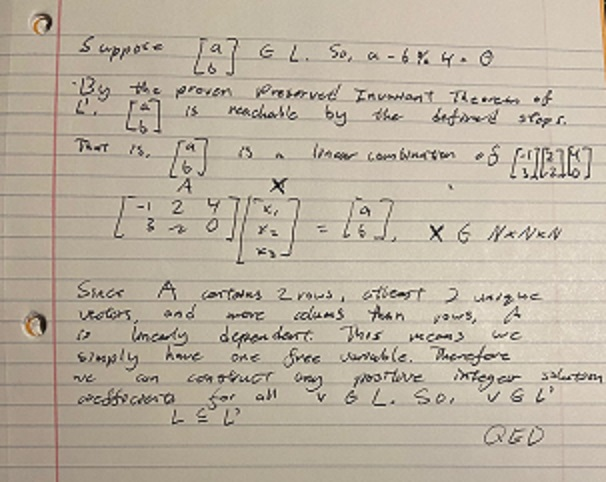
\includegraphics{6c.jpg}
        \end{enumerate}
    \end{enumerate}


    \noindent
    For more practice, work on the problems from Rosen Sections 5.3; Lehman et al. Chapters 5, 6.1 - 6.2, 7

\end{document}

